%%%%%%%%%%%%%%%%%%%%%%%%%%%%%%%%%%%%%%%%%
% Masters/Doctoral Thesis 
% LaTeX Template
% Version 2.4 (22/11/16)
%
% This template has been downloaded from:
% http://www.LaTeXTemplates.com
%
% Version 2.x major modifications by:
% Vel (vel@latextemplates.com)
%
% This template is based on a template by:
% Steve Gunn (http://users.ecs.soton.ac.uk/srg/softwaretools/document/templates/)
% Sunil Patel (http://www.sunilpatel.co.uk/thesis-template/)
%
% Template license:
% CC BY-NC-SA 3.0 (http://creativecommons.org/licenses/by-nc-sa/3.0/)
%
%%%%%%%%%%%%%%%%%%%%%%%%%%%%%%%%%%%%%%%%%

%----------------------------------------------------------------------------------------
%	PACKAGES AND OTHER DOCUMENT CONFIGURATIONS
%----------------------------------------------------------------------------------------

\documentclass[
  12pt, % The default document font size, options: 10pt, 11pt, 12pt
  %oneside, % Two side (alternating margins) for binding by default, uncomment to switch to one side
  %chapterinoneline,% Have the chapter title next to the number in one single line
  english, % ngerman for German
  doublespacing, % Single line spacing, alternatives: singlespacing, onehalfspacing or doublespacing
  %draft, % Uncomment to enable draft mode (no pictures, no links, overfull hboxes indicated)
  %nolistspacing, % If the document is onehalfspacing or doublespacing, uncomment this to set spacing in lists to single
  %liststotoc, % Uncomment to add the list of figures/tables/etc to the table of contents
  %toctotoc, % Uncomment to add the main table of contents to the table of contents
  %parskip, % Uncomment to add space between paragraphs
  %nohyperref, % Uncomment to not load the hyperref package
  %headsepline, % Uncomment to get a line under the header
]{setting} % The class file specifying the document structure

\usepackage[utf8]{inputenc} % Required for inputting international characters
\usepackage[T1]{fontenc} % Output font encoding for international characters
\usepackage{amssymb}
\usepackage{palatino} % Use the Palatino font by default

\usepackage[backend=bibtex,style=authoryear,natbib=true]{biblatex} % Use the bibtex backend with the authoryear citation style (which resembles APA)

\addbibresource{example.bib} % The filename of the bibliography

\usepackage[autostyle=true]{csquotes} % Required to generate language-dependent quotes in the bibliography

%----------------------------------------------------------------------------------------
%	MARGIN SETTINGS
%----------------------------------------------------------------------------------------

\geometry{
  paper=a4paper, % Change to letterpaper for US letter
  inner=2.0cm, % Inner margin 2.5cm
  outer=2.2cm, % Outer margin 3.8cm
  bindingoffset=2cm, % Binding offset
  top=1.5cm, % Top margin
  bottom=1.5cm, % Bottom margin
  %showframe,% show how the type block is set on the page
}

%----------------------------------------------------------------------------------------
%	THESIS INFORMATION
%----------------------------------------------------------------------------------------

\thesistitle{Thesis Title} % Your thesis title, this is used in the title and abstract, print it elsewhere with \ttitle
\supervisor{Dr. James \textsc{Smith}} % Your supervisor's name, this is used in the title page, print it elsewhere with \supname
\examiner{} % Your examiner's name, this is not currently used anywhere in the template, print it elsewhere with \examname
\degree{Doctor of Philosophy} % Your degree name, this is used in the title page and abstract, print it elsewhere with \degreename
\author{John \textsc{Smith}} % Your name, this is used in the title page and abstract, print it elsewhere with \authorname
\addresses{} % Your address, this is not currently used anywhere in the template, print it elsewhere with \addressname

\subject{Biological Sciences} % Your subject area, this is not currently used anywhere in the template, print it elsewhere with \subjectname
\keywords{} % Keywords for your thesis, this is not currently used anywhere in the template, print it elsewhere with \keywordnames
\university{\href{http://www.university.com}{University Name}} % Your university's name and URL, this is used in the title page and abstract, print it elsewhere with \univname
\department{\href{http://department.university.com}{Department or School Name}} % Your department's name and URL, this is used in the title page and abstract, print it elsewhere with \deptname
\group{\href{http://researchgroup.university.com}{Research Group Name}} % Your research group's name and URL, this is used in the title page, print it elsewhere with \groupname
\faculty{\href{http://faculty.university.com}{Faculty Name}} % Your faculty's name and URL, this is used in the title page and abstract, print it elsewhere with \facname

\AtBeginDocument{
\hypersetup{pdftitle=\ttitle} % Set the PDF's title to your title
\hypersetup{pdfauthor=\authorname} % Set the PDF's author to your name
\hypersetup{pdfkeywords=\keywordnames} % Set the PDF's keywords to your keywords
}

\begin{document}

\frontmatter % Use roman page numbering style (i, ii, iii, iv...) for the pre-content pages

\pagestyle{plain} % Default to the plain heading style until the thesis style is called for the body content

%----------------------------------------------------------------------------------------
%	TITLE PAGE
%----------------------------------------------------------------------------------------

\begin{titlepage}
\begin{center}

\vspace*{.06\textheight}
{\scshape\LARGE \univname\par}\vspace{1.5cm} % University name
\textsc{\Large Doctoral Thesis}\\[0.5cm] % Thesis type

\HRule \\[0.4cm] % Horizontal line
{\huge \bfseries \ttitle\par}\vspace{0.4cm} % Thesis title
\HRule \\[1.5cm] % Horizontal line
 
\begin{minipage}[t]{0.4\textwidth}
\begin{flushleft} \large
\emph{Author:}\\
\href{http://www.johnsmith.com}{\authorname} % Author name - remove the \href bracket to remove the link
\end{flushleft}
\end{minipage}
\begin{minipage}[t]{0.4\textwidth}
\begin{flushright} \large
\emph{Supervisor:} \\
\href{http://www.jamessmith.com}{\supname} % Supervisor name - remove the \href bracket to remove the link  
\end{flushright}
\end{minipage}\\[3cm]
 
\vfill

\large \textit{A thesis submitted in fulfillment of the requirements\\ for the degree of \degreename}\\[0.3cm] % University requirement text
\textit{in the}\\[0.4cm]
\groupname\\\deptname\\[2cm] % Research group name and department name
 
\vfill

{\large \today}\\[4cm] % Date
%\includegraphics{Logo} % University/department logo - uncomment to place it
 
\vfill
\end{center}
\end{titlepage}

%----------------------------------------------------------------------------------------
%	DECLARATION PAGE
%----------------------------------------------------------------------------------------

\begin{declaration}
\addchaptertocentry{\authorshipname} % Add the declaration to the table of contents
\noindent I, \authorname, declare that this thesis titled, \enquote{\ttitle} and the work presented in it are my own. I confirm that:

\begin{itemize} 
\item This work was done wholly or mainly while in candidature for a research degree at this University.
\item Where any part of this thesis has previously been submitted for a degree or any other qualification at this University or any other institution, this has been clearly stated.
\item Where I have consulted the published work of others, this is always clearly attributed.
\item Where I have quoted from the work of others, the source is always given. With the exception of such quotations, this thesis is entirely my own work.
\item I have acknowledged all main sources of help.
\item Where the thesis is based on work done by myself jointly with others, I have made clear exactly what was done by others and what I have contributed myself.\\
\end{itemize}
 
\noindent Signed:\\
\rule[0.5em]{25em}{0.5pt} % This prints a line for the signature
 
\noindent Date:\\
\rule[0.5em]{25em}{0.5pt} % This prints a line to write the date
\end{declaration}

\cleardoublepage

%----------------------------------------------------------------------------------------
%	QUOTATION PAGE
%----------------------------------------------------------------------------------------

\vspace*{0.2\textheight}

\noindent\enquote{\itshape Thanks to my solid academic training, today I can write hundreds of words on virtually any topic without possessing a shred of information, which is how I got a good job in journalism.}\bigbreak

\hfill Dave Barry

%----------------------------------------------------------------------------------------
%	ABSTRACT PAGE
%----------------------------------------------------------------------------------------

\begin{abstract}
\addchaptertocentry{\abstractname} % Add the abstract to the table of contents
The Thesis Abstract is written here (and usually kept to just this page). The page is kept centered vertically so can expand into the blank space above the title too\ldots
\end{abstract}

%----------------------------------------------------------------------------------------
%	ACKNOWLEDGEMENTS
%----------------------------------------------------------------------------------------

\begin{acknowledgements}
\addchaptertocentry{\acknowledgementname} % Add the acknowledgements to the table of contents
The acknowledgments and the people to thank go here, don't forget to include your project advisor\ldots
\end{acknowledgements}

%----------------------------------------------------------------------------------------
%	LIST OF CONTENTS/FIGURES/TABLES PAGES
%----------------------------------------------------------------------------------------

\tableofcontents % Prints the main table of contents

\listoffigures % Prints the list of figures

\listoftables % Prints the list of tables

%----------------------------------------------------------------------------------------
%	ABBREVIATIONS
%----------------------------------------------------------------------------------------

\begin{abbreviations}{ll} % Include a list of abbreviations (a table of two columns)

\textbf{LAH} & \textbf{L}ist \textbf{A}bbreviations \textbf{H}ere\\
\textbf{WSF} & \textbf{W}hat (it) \textbf{S}tands \textbf{F}or\\

\end{abbreviations}

%----------------------------------------------------------------------------------------
%	PHYSICAL CONSTANTS/OTHER DEFINITIONS
%----------------------------------------------------------------------------------------

\begin{constants}{lr@{${}={}$}l} % The list of physical constants is a three column table

% The \SI{}{} command is provided by the siunitx package, see its documentation for instructions on how to use it

Speed of Light & $c_{0}$ & \SI{2.99792458e8}{\meter\per\second} (exact)\\
%Constant Name & $Symbol$ & $Constant Value$ with units\\

\end{constants}

%----------------------------------------------------------------------------------------
%	SYMBOLS
%----------------------------------------------------------------------------------------

\begin{symbols}{lll} % Include a list of Symbols (a three column table)

$a$ & distance & \si{\meter} \\
$P$ & power & \si{\watt} (\si{\joule\per\second}) \\
%Symbol & Name & Unit \\

\addlinespace % Gap to separate the Roman symbols from the Greek

$\omega$ & angular frequency & \si{\radian} \\

\end{symbols}

%----------------------------------------------------------------------------------------
%	DEDICATION
%----------------------------------------------------------------------------------------

\dedicatory{For/Dedicated to/To my\ldots} 

%----------------------------------------------------------------------------------------
%	THESIS CONTENT - CHAPTERS
%----------------------------------------------------------------------------------------

\mainmatter % Begin numeric (1,2,3...) page numbering

\pagestyle{thesis} % Return the page headers back to the "thesis" style

% Include the chapters of the thesis as separate files from the Chapters folder
% Uncomment the lines as you write the chapters

%\chapter{Introduction and Theory Overview} \label{chap:1}

\section{Introduction}
The analysis is aim at searching for heavy resonances decaying to a pair of Higgs
bosons in the four b quark final state using 35.9$fb^{-1}$ proton-proton collison data at center-of-mass energy 13 TeV collected with the CMS detector at the LHC. The figure 1.1 shows the feynman diagram of the channel. 

The Higgs tagging process uses the b-tagging algorithm, N-subjetness variable, and the mass of the jets. The analysis is searching for a bump in the dominant background of multi-jet events.


\begin{figure}[t]
  \begin{center}

    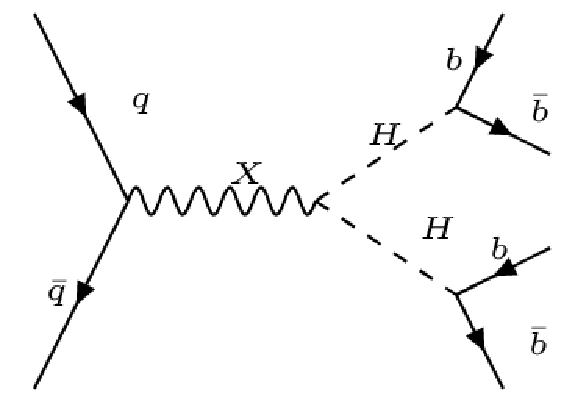
\includegraphics[width=0.5\textwidth]{Figures/Screenshot_20170601_160641.pdf} 
    \end{center}
  \caption{The feynman diagram of q$\bar{q}$ $\rightarrow$ X $\rightarrow$ HH $\rightarrow$ $b\bar{b}b\bar{b}$.}
\end{figure}

In \autoref{chap:1}, an overview of Wrapped Extra Dimension theory, signal model, and motivation is presented. In \autoref{chap:2}, the LHC and the CMS detector are simply introduced. In \autoref{chap:3}, the information of the data and the Monte Carlo Simulation is shown along with the comparison of shape of each discripant variable. The reconstruction and the selection of the event is also fully detailed. In \autoref{chap:4}, the background estimation method based on data driven is presented. All sysyematic uncertainted considered is documented in \autoref{chap:5}. Finally, the result of 95$\% $ CL$_{s}$ upper limit of cross section $\times$ branch ratio is shwon in \autoref{chap:6}. 

\section{Theory}
%http://dx.doi.org/10.1016/j.physletb.2012.08.021
%http://www.sciencedirect.com/science/article/pii/S037026931200857X

The discovery of the boson whose mass around 125 GeV and with properties close to Higgs mechanism in the Standard model has incited the search under Higgs potential including Higgs self-coupling\citep{jetarea_fastjet_pu,HiggsdiscoveryAtlas}. Especially, it is a worth explored channel to finding new physic beyond Standard model. 
Targeting heavy resonance, the model Wrapped Extra Dimension is considered. 

\subsection{Wraped Extra Dimension} 

%https://journals.aps.org/prl/pdf/10.1103/PhysRevLett.83.3370
To solve the hierarchy problem, Wrapped Extra dimension proposed by Randall and Sundrum postulates a scenario that the SM particles and forces associating with gravity force are confined to a four-dimension subspace within (4+n)-dimension spacetime, referred to as "3-brane", 
to explain the fact that we do not see experimental signs of the extra dimensions\citep{Randall:1999ee}.  The spacetime metrix takes the form\citep{Oliveira:2014kla}:

\begin{equation} \label{eq1}
\begin{split}
ds^2 = e^{-2\sigma(\phi)}\eta_{\mu\nu}dx^{\mu}dx^{\nu} + r^2_{c}d\phi^2, 
\end{split}
\end{equation}
where $\mu$ and $\nu$ run over 1, 2, 3, and 4, and $\phi$ is the fifth dimension. Its classical action is 

\begin{equation} \label{eq1}
\begin{split}
S = S_{Gravity}+S_{TeV}+S_{Planck}+S_{Matter},
\end{split}
\end{equation},
where $S_{Gravity}$ is the action of bulk gravity, and $S_{Matter}$ is the action of matter field. The actions can be written as:

\begin{equation} \label{eq1}
\begin{split}
S_{i=TeV/Planck}=-\int d^4x \sqrt{g(\phi =0,\pi)}\Lambda_{i=TeV/Planck}\\
S_{Gravity}=\int d^4 \int ^{\pi}_{\pi} d\phi \sqrt{g}(-\Lambda_{bulk}+2M^3_{5}R),
\end{split}
\end{equation}
where $\Lambda$ is hte vacuum energy density, R is Ricci metrix. We arrive at:

\begin{equation} \label{eq1}
\begin{split}
\sigma(\phi)=r_{c}|\phi | \sqrt{\frac{-\Lambda}{24M^2_5}}\equiv r_c|\phi |k \\
k\equiv  \sqrt{\frac{-\Lambda}{24M^2_5}}, \\
\end{split}
\end{equation}
where k is referred as curvature factor. We can integrate the fifth dimension and get four-dimension Planck mass: 
\begin{equation} \label{eq1}
\begin{split}
\bar{M}^2_{Pl}=\frac{M^3_5}{k}(1=e^{-2\pi kr_c}).
\end{split}
\end{equation}

Finally, we get the spacetime metrix:  
\begin{equation} \label{eq1}
\begin{split}
ds^2 = e^{-2kr_c\phi}\eta_{\mu\nu}dx^{\mu}dx^{\nu} + r^2_{c}d\phi^2, 
\end{split}
\end{equation}


where k is a scale of the order of the Planck scale, xm are
coordinates for the familiar four dimensions, while 0 $\leq$ $\phi$ $\leq$ $\pi$ is the coordinate for an extra dimension, which is
a finite interval whose size is set by $r_c$. The exponential is the source of large hierarchy between weak and the observed Planck scale.  


%https://journals.aps.org/prl/pdf/10.1103/PhysRevLett.83.4922
%https://arxiv.org/pdf/hep-ph/9911406.pdf

%https://arxiv.org/pdf/hep-ph/9909255.pdf
%https://arxiv.org/pdf/hep-ph/0701186.pdf
%https://arxiv.org/pdf/hep-ph/0701150.pdf
There are models predicting the existence of new particles, such as spin-0 radion and spin-2 graviton\citep{Davoudiasl:1999jd,Agashe:2007zd,Fitzpatrick:2007qr}. For example, a radion scalar is added to stablize the $r_c$ in RS theory without a fune-tuning of parameters\citep{Goldberger:1999uk}. Other model proves that
a radion field can remove the constraints between two branes without a stablized radius\citep{Csaki:1999mp}, and that 
%https://arxiv.org/pdf/hep-th/0008151.pdf
a radion scalar can exist with radus stabilization in bulk scalar field while assuming stabilization exists\citep{Csaki:2000zn}.
A possible mixing of the radion which is the only graviscalar in RS model and the Higgs is proposed\citep{Giudice:2000av}.
%https://arxiv.org/pdf/hep-ph/0002178.pdf
However, according to the latest experimental data, the mixing is expected to be small. Therefore, the contribution of the mixing is not considered in this analysis\citep{Desai:2013pga}.
%https://arxiv.org/pdf/1307.3765.pdf

We follow the ref.\citep{Agashe:2013kyb} to calculate the cross section of bulk graviton.
\begin{equation} \label{eq1}
\begin{split}
gg \rightarrow KK graviton \rightarrow ZZ, WW, hh (and t\bar{t}, b\bar{b}) \\
\textit{L}_{prod.} = 0.053 (\frac{k}{M_{Pl}M_{G}})\eta^{\mu\alpha}\eta^{\nu\beta}h^{(1)}_{\alpha\beta}T^{gluon}_{\mu \nu}(x), 
\end{split}
\end{equation}
where the $M_G$ is the mass of KK graviton, and $T^{gluon}_{\mu \nu}$ is four-dimesion four-momentum of SM gluon. The implementation of the calcuation is described in ref.\citep{Oliveira:2014kla}. The model which is capable of calculating the correction of next-to-leading-order QCD induced spin-2 particle is used. The cross section is calculated by \textsf{MG5\_aMC@NLO}.
Because of the Higgs-like property of radion, the cross section of radion is calculated by rescaling the cross section of Higgs like particle\citep{Agashe:2013kyb,AN-16-300}. The production of Higgs-like particle by gluon-gluon fusion is followed by ref.\citep{Catani:2003zt,Heinemeyer:2013tqa}, which is calcuated in next-to-next-to-leading-order QCD induced soft-gluon resummation. The Higgs-like calculation is up to 1 TeV, and it is constant for mass above 1 TeV. The cross section of radion is based on the cross section of Higgs-like multiplied by k factor. 
In the calcuation of both signal, CTEQ6LPDF is used\citep{Nadolsky:2008zw}.  

\subsection{Motivation} 
%https://arxiv.org/pdf/1512.04357.pdf
There are models predicting heavy resonances decaying into VV\citep{Brehmer:2015dan}.
%https://arxiv.org/abs/1506.00962
%https://arxiv.org/abs/1503.04677
%https://arxiv.org/abs/1409.6190
%https://arxiv.org/abs/1405.1994
Several researches on these channels are performed in both CMS and ATLAS.
There are also the combinations of these analyses\citep{Khachatryan:2014hpa,ATLASZV,ATLASWV,ATLASVV}.
%https://arxiv.org/abs/1405.3447
%https://arxiv.org/abs/1512.05099
The combination from ATLAS excludes the resonance of Bulk Graviton from below 810 GeV\citep{Aad:2015ipg}, and despit the combination from CMS fails to exclude any mass spectum of Bulk Graviton given a less sensitive model, it sets the upper limit of 10 fb of cross section of Bulk Graviton through $M_X$ from 600 to 2500 GeV\citep{CMSZVWV}.
%https://arxiv.org/pdf/1503.04114.pdf
%https://arxiv.org/pdf/1506.00285.pdf
Besides, searches for Bulk Graviton decaying into HH in four b-flavored quarks final state have been perfromed by CMS and ATLAS at $\sqrt{s}$ = 8 TeV\citep{Khachatryan:2015year,Aad:2015uka}. They exlude the mass region below 830 and 720 GeV respectively. The intermediate region of the mass of heavy resonances ( $M_X \thickapprox$ 2 TeV ) is left interesting to be explored.
 



%
%\begin{figure}[t]
%  \centering
%  \begin{tabular}{cc}
%    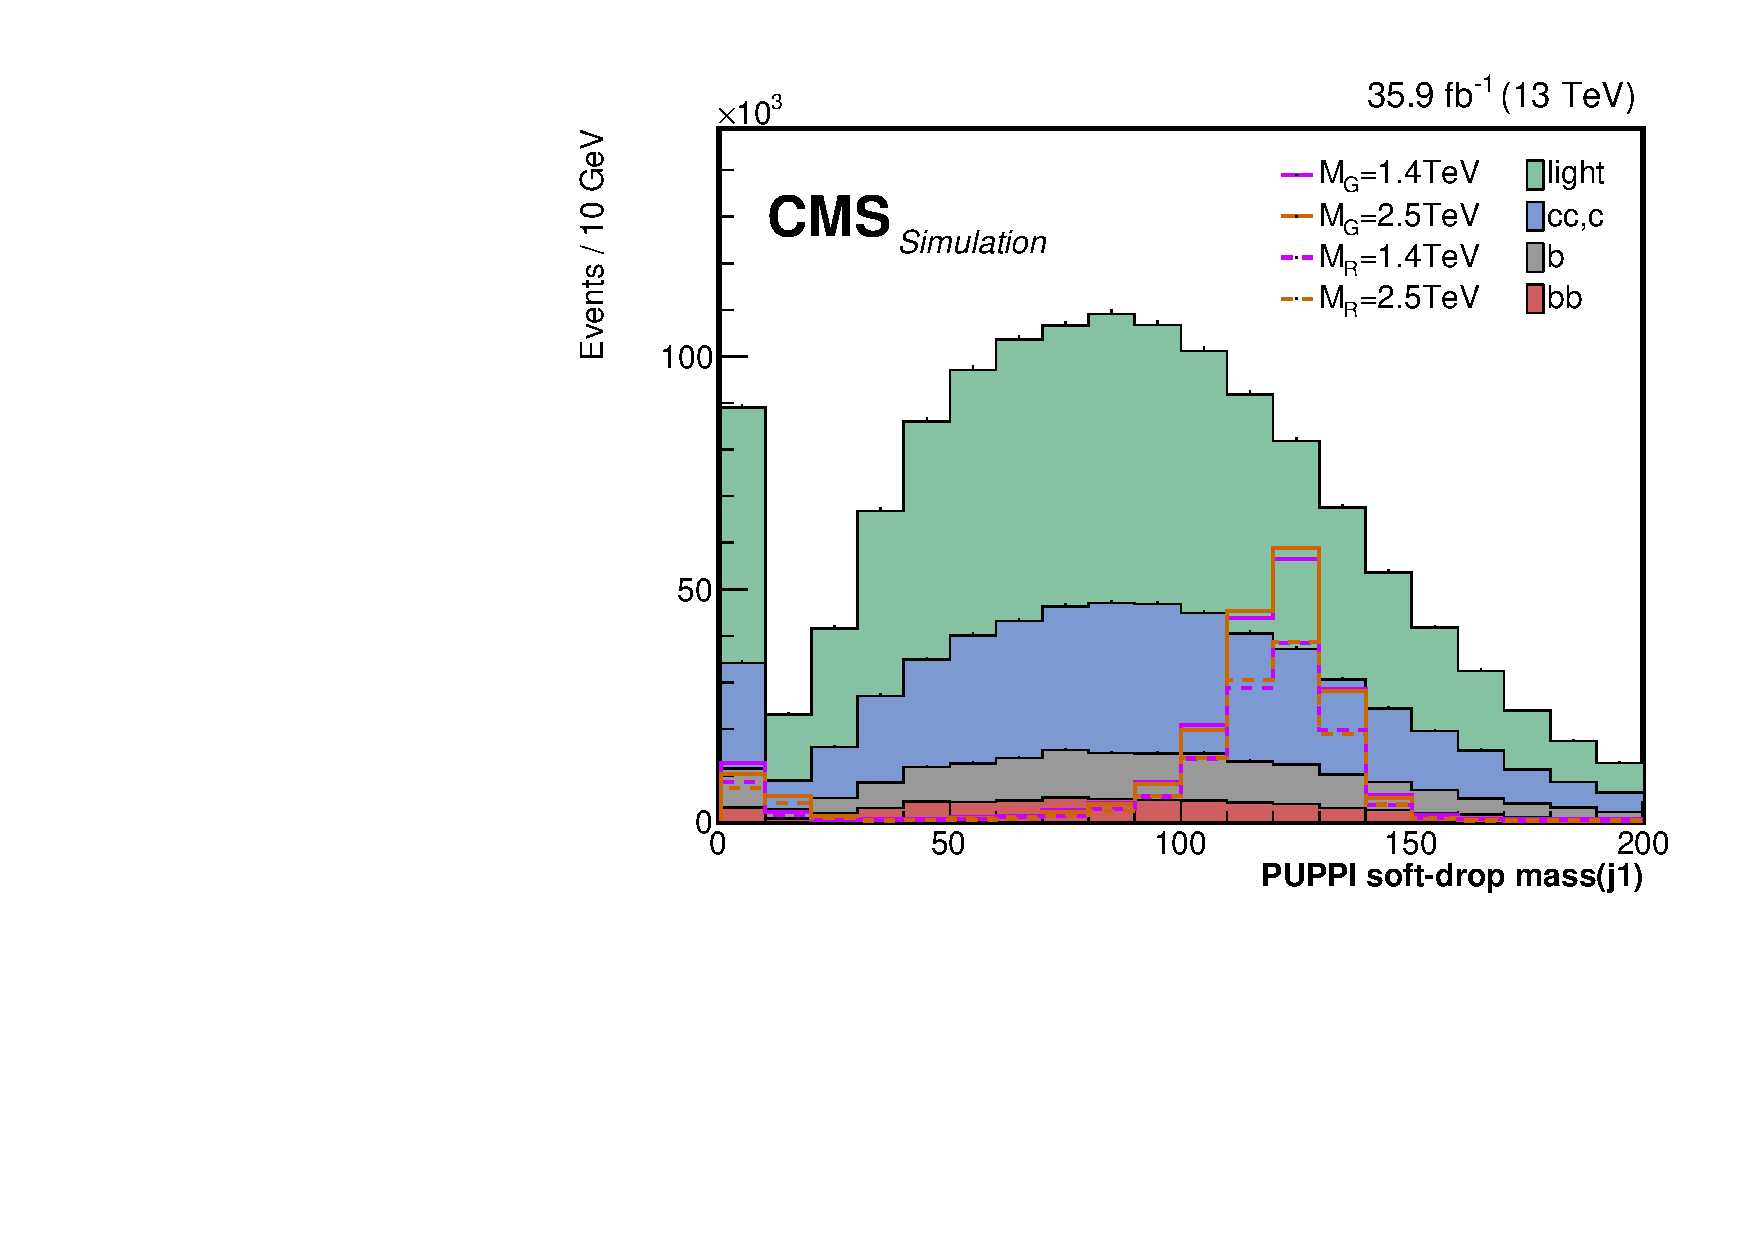
\includegraphics[width=0.5\textwidth]{Figures/MC_N1/puppiSDMassThea_j0.pdf} &
%    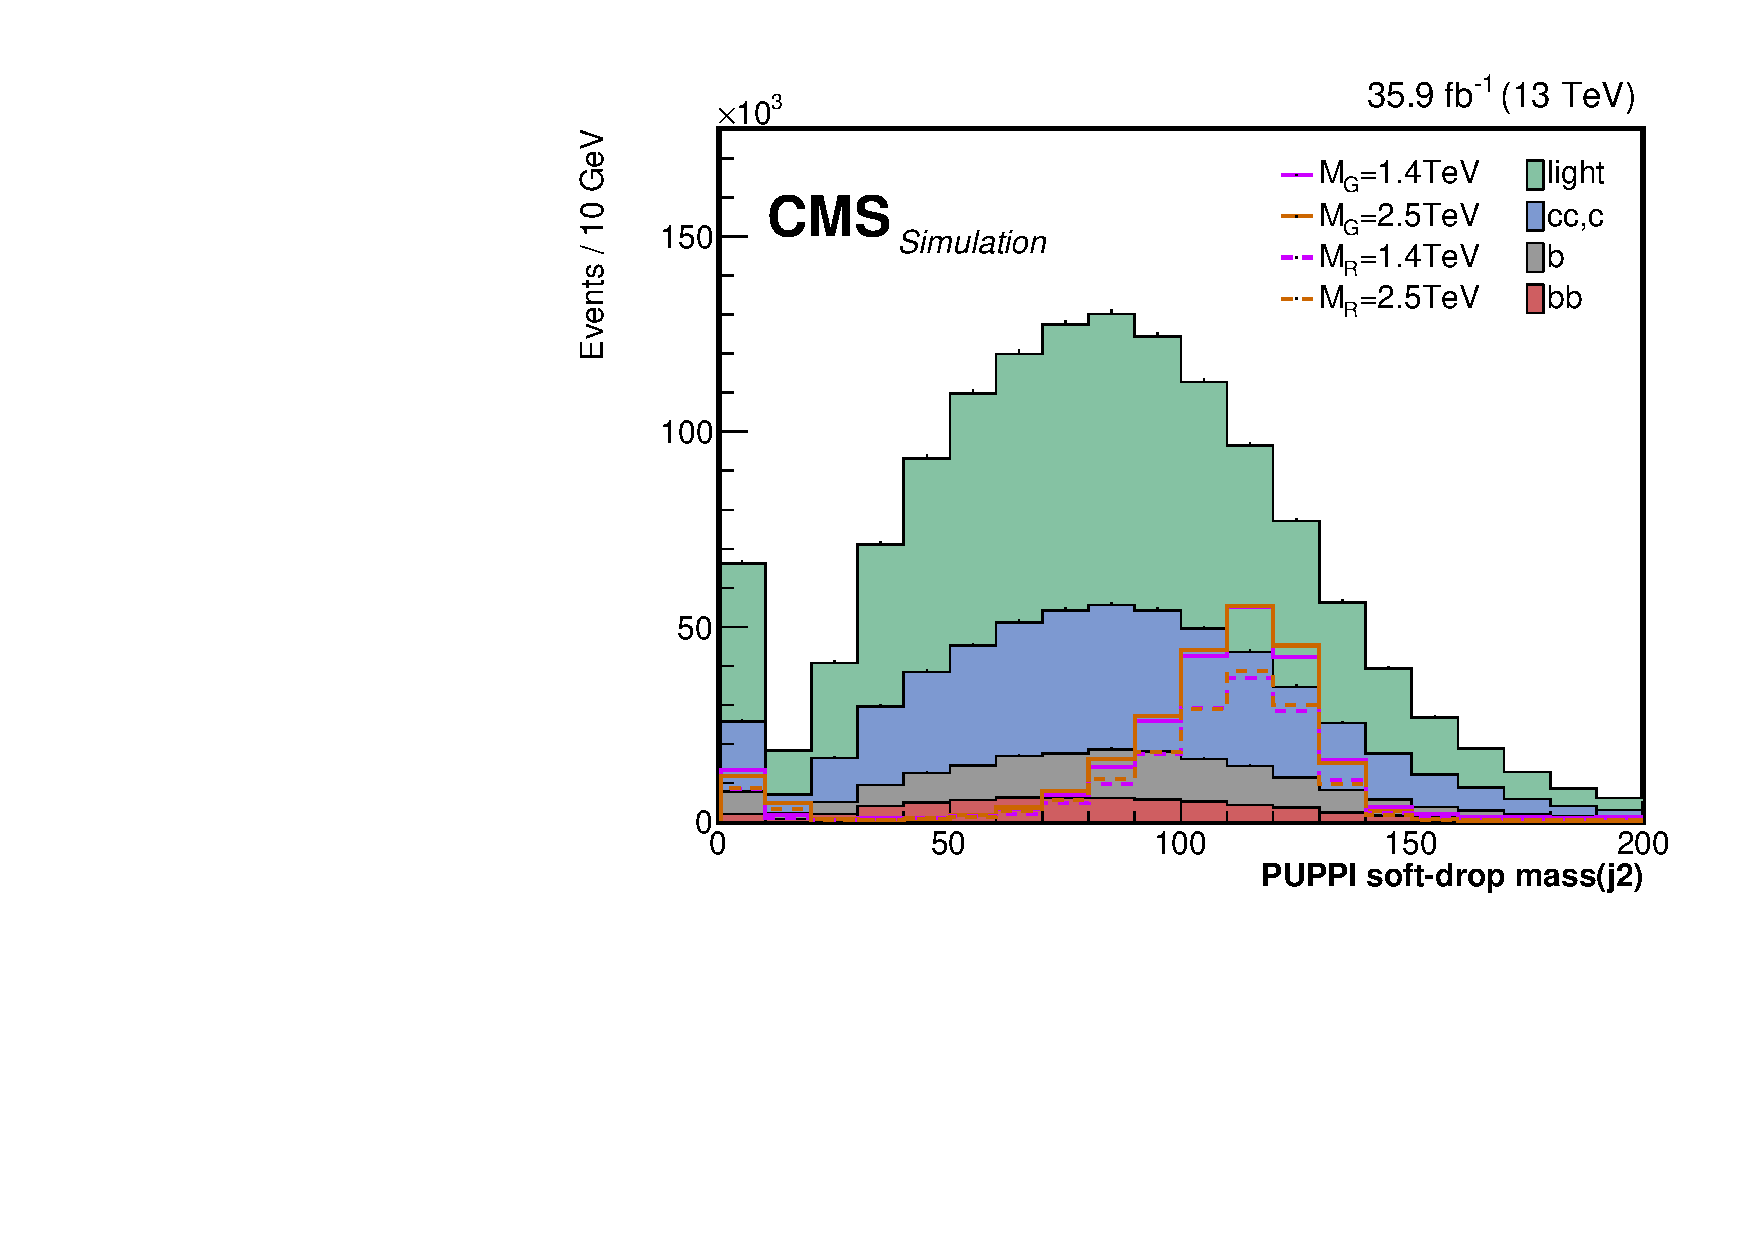
\includegraphics[width=0.5\textwidth]{Figures/MC_N1/puppiSDMassThea_j1.pdf} \\
%     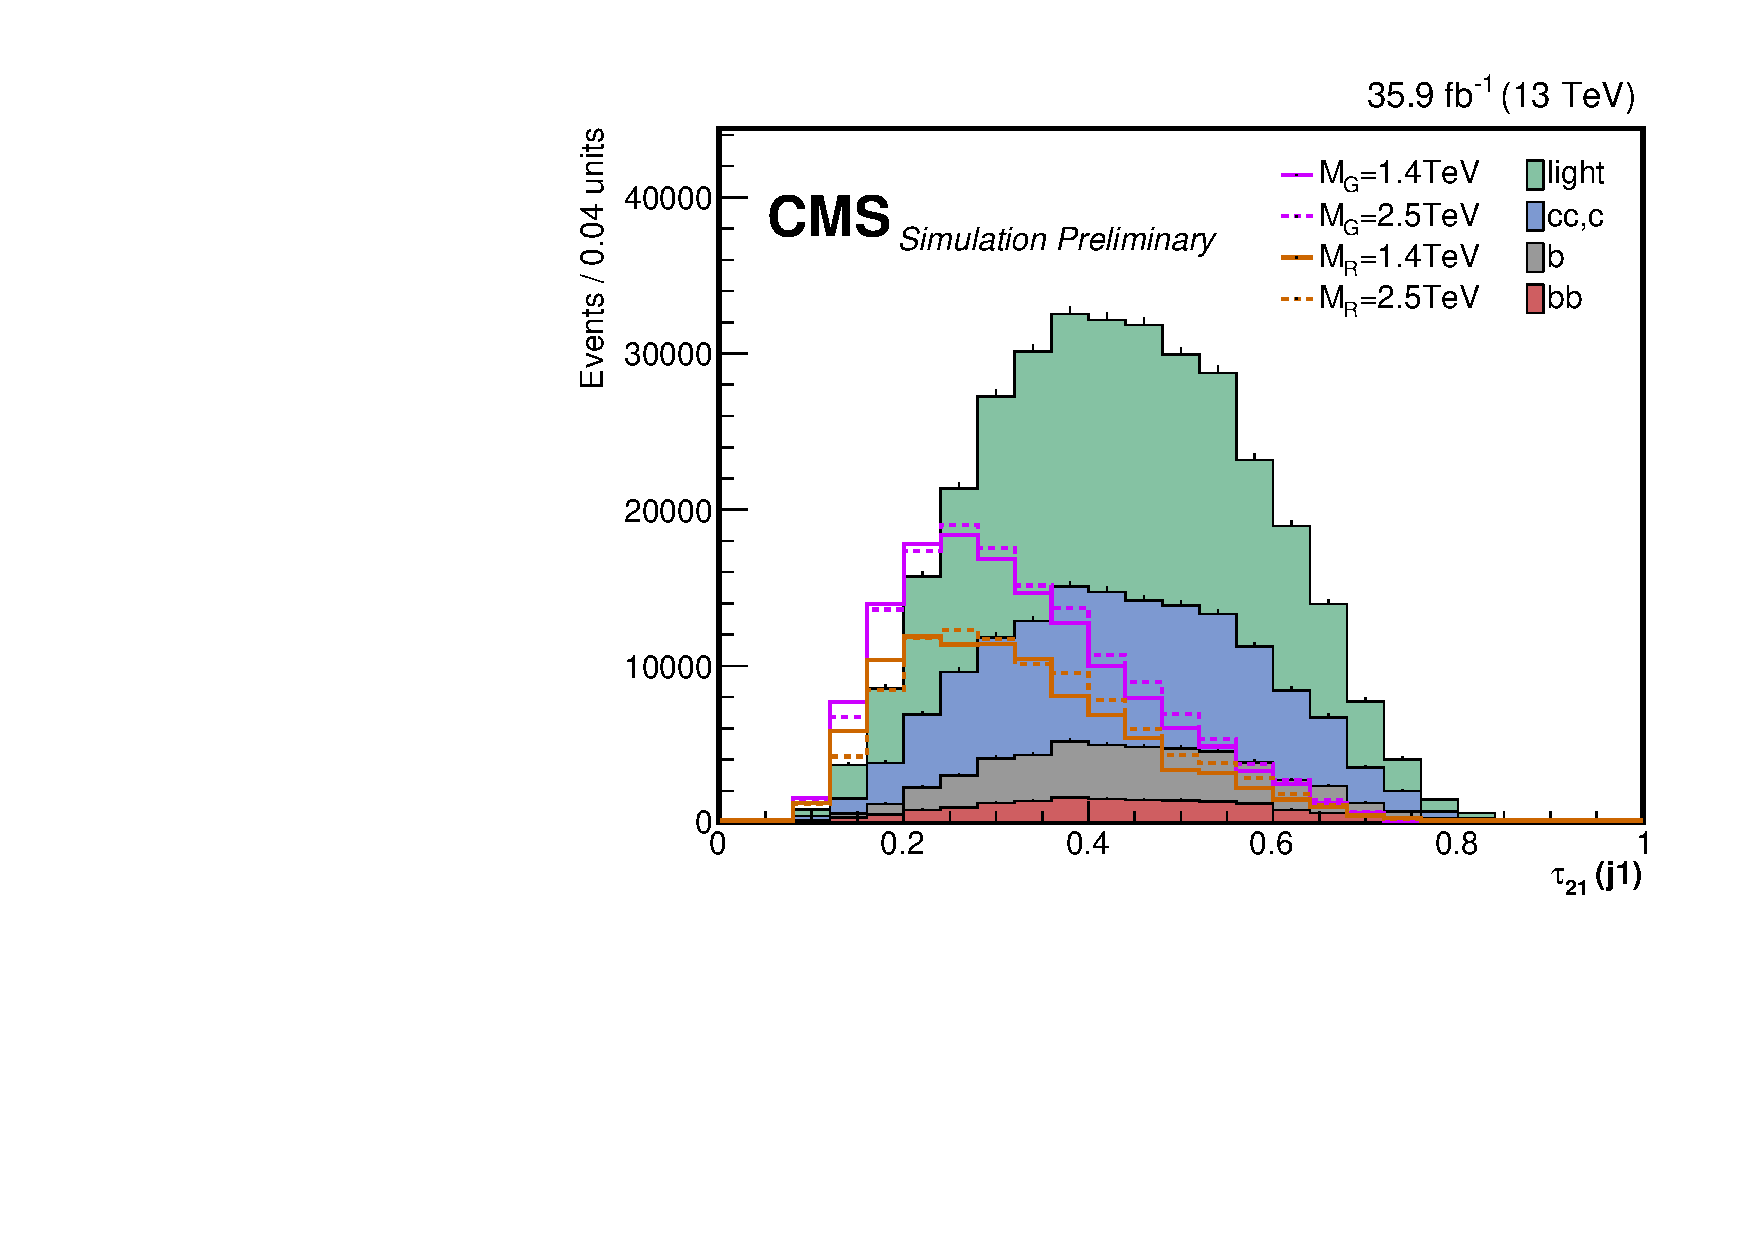
\includegraphics[width=0.5\textwidth]{Figures/MC_N1/puppiTau21_j0.pdf} &
%    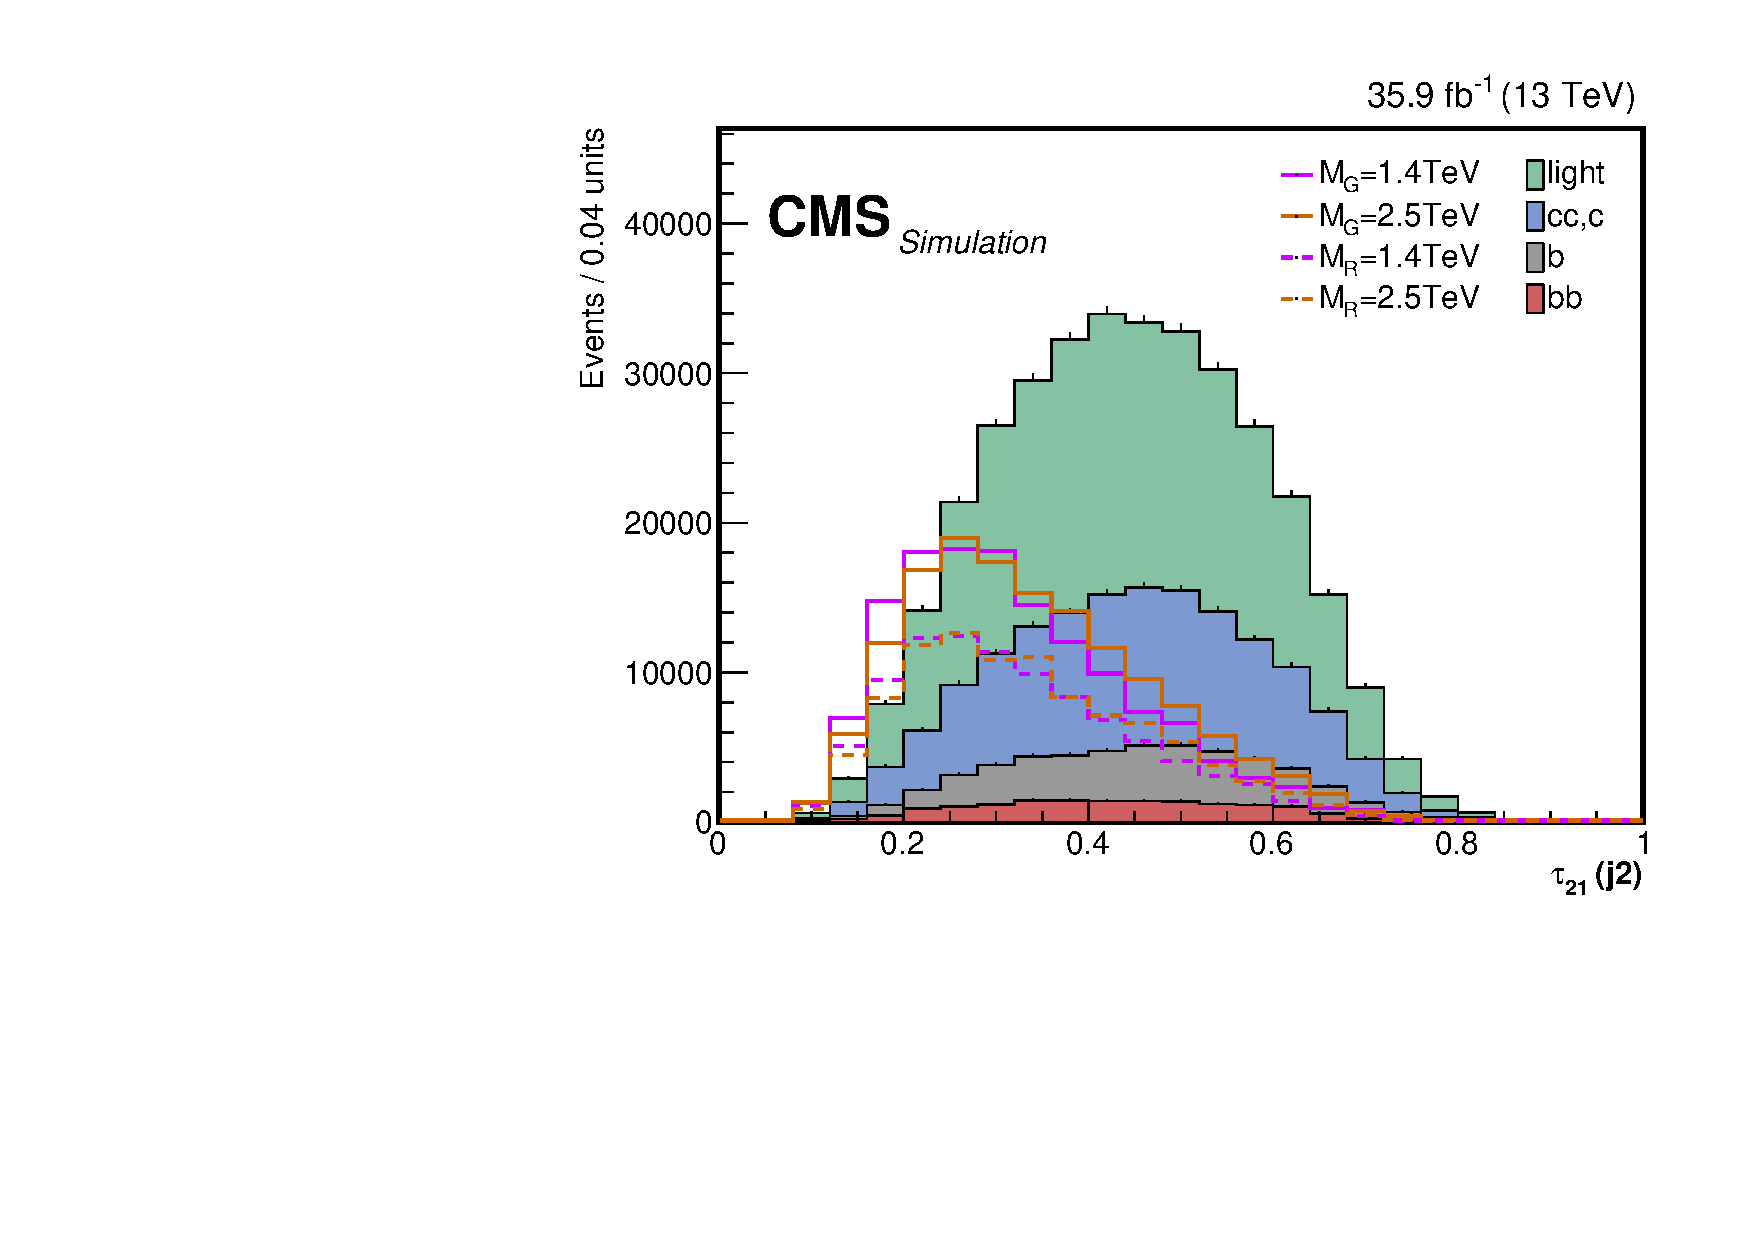
\includegraphics[width=0.5\textwidth]{Figures/MC_N1/puppiTau21_j1.pdf} \\
%     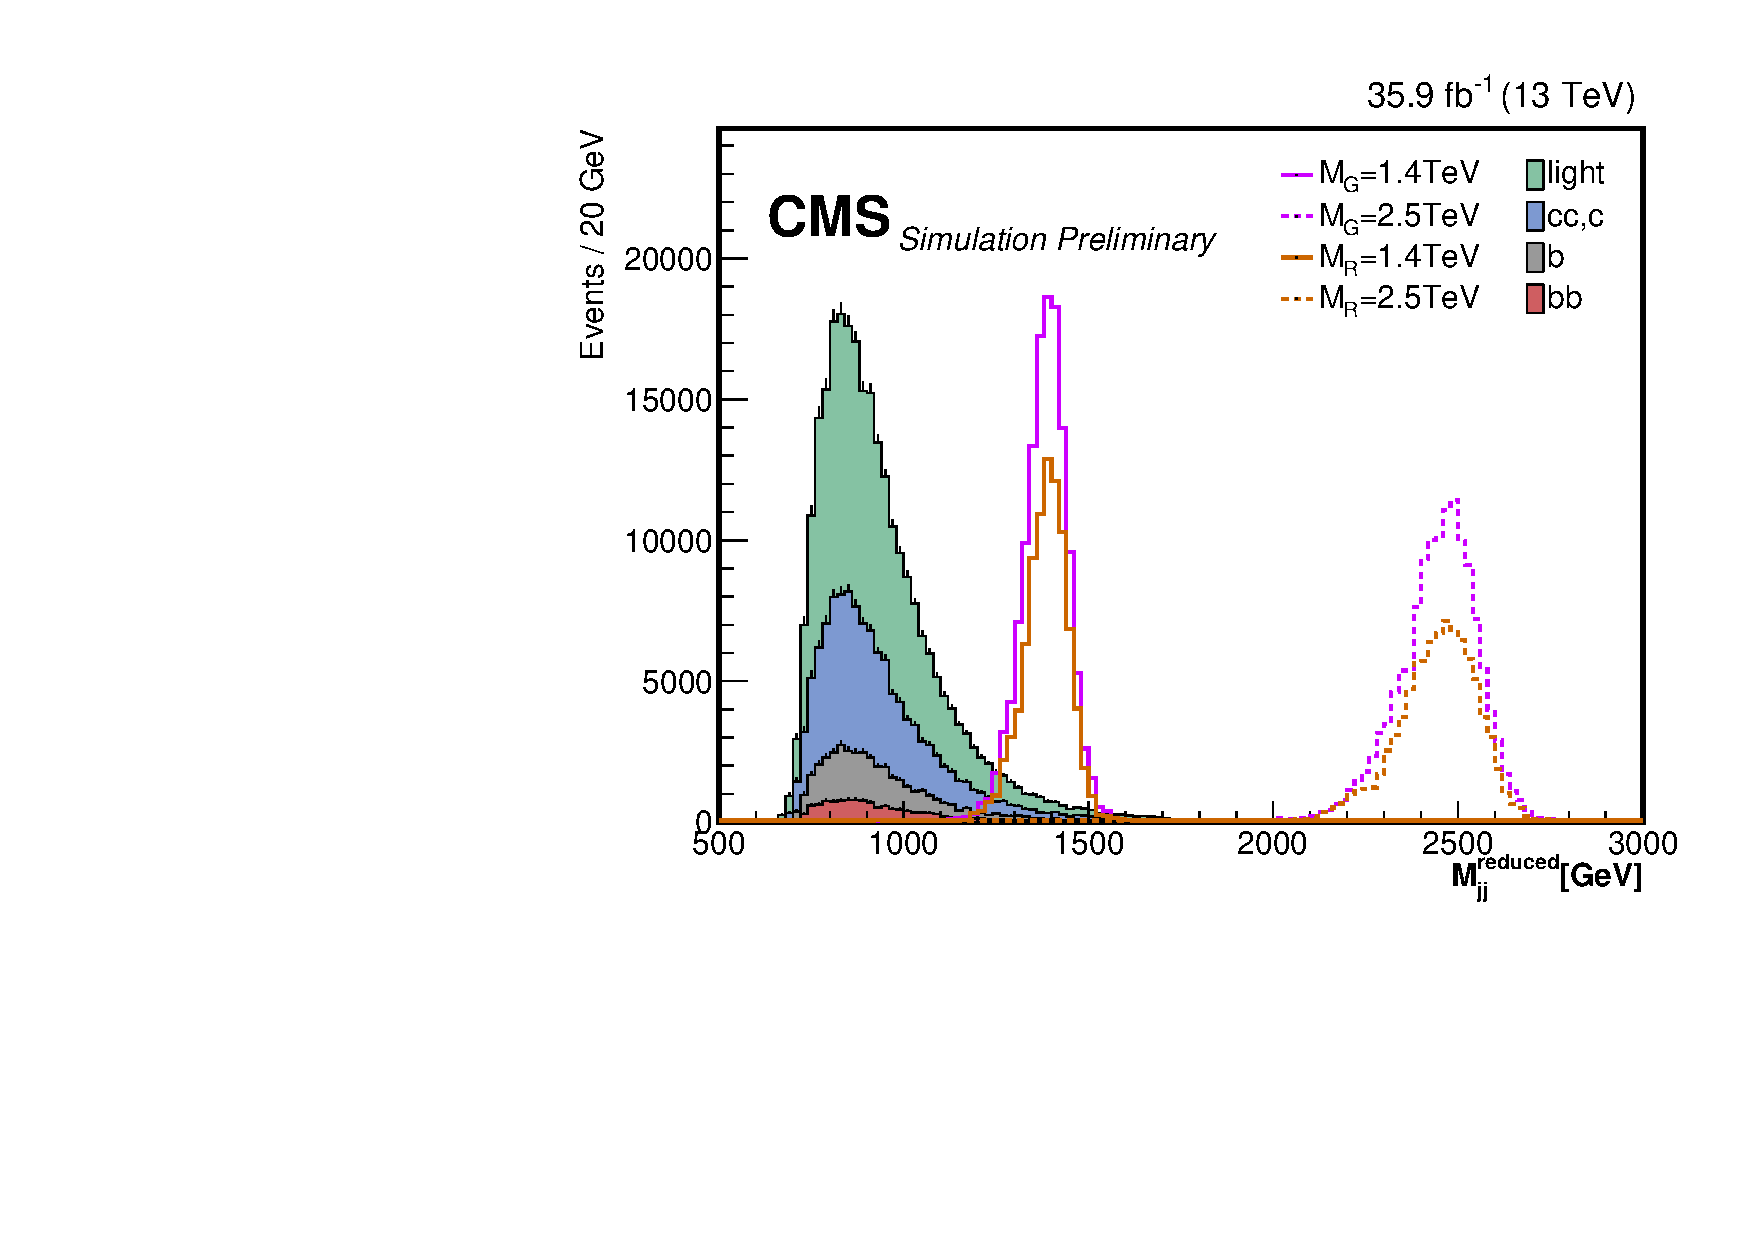
\includegraphics[width=0.5\textwidth]{Figures/MC_N1/totalMassRed.pdf} &
%    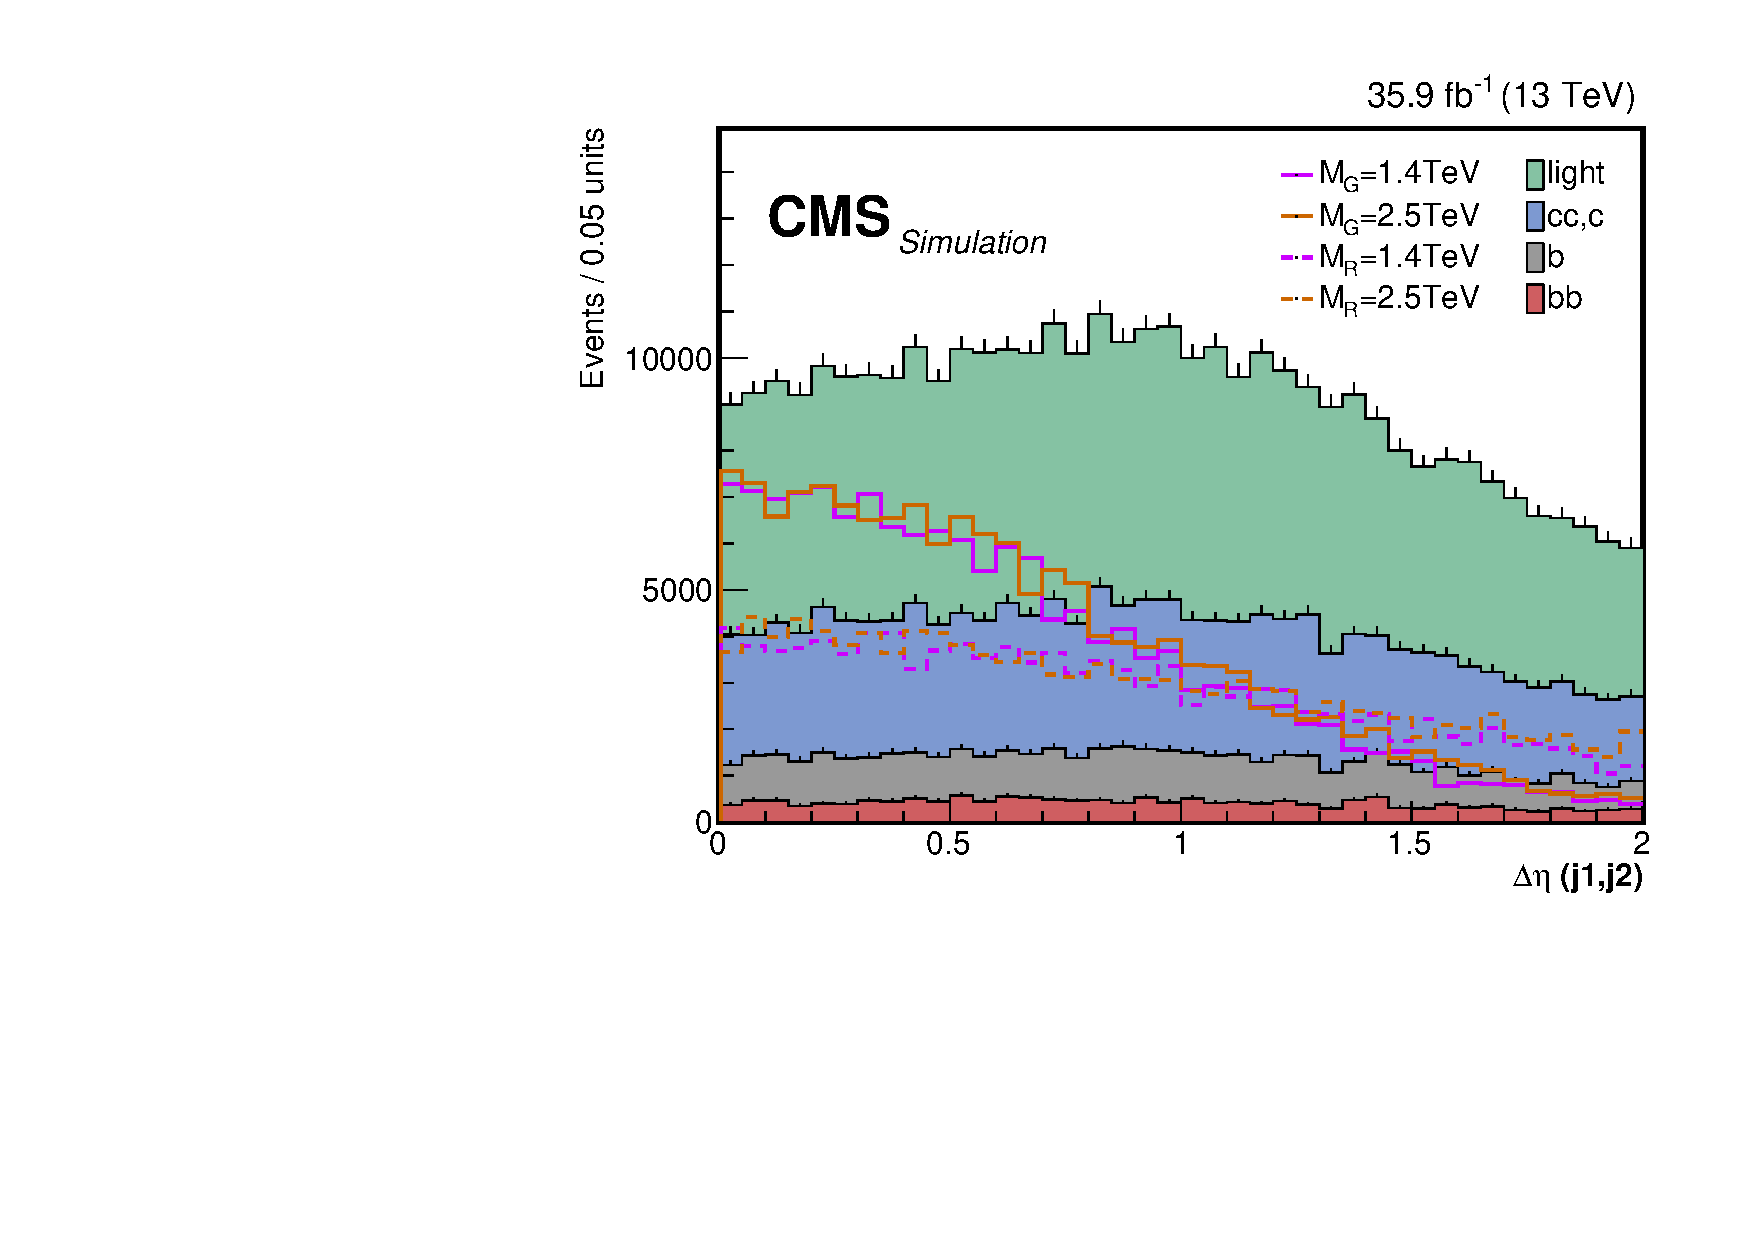
\includegraphics[width=0.5\textwidth]{Figures/MC_N1/deltaEta.pdf} \\
%  \end{tabular}
%  \caption{The comparison of signal and background. The signals of $M_{X}$ = 1.4 TeV and 2.5 TeV from both models are shown. The cross section is set to 20 pb in the figures. Multi-jet events are seperated into four categories summarized in the table 2.10. From top to buttom are the comparison of PUPPI soft-drop mass, $\tau _{21}$ of leading (left) and next leading (right) AK8 jet, the reduced mass (buttom left), and |$\Delta \eta $ (the two leading AK8 jets)| (buttom right).}
%  \label{fig:hvt_brs}
%\end{figure}
% Chapter 1

\newcommand{\tabhead}[1]{\textbf{#1}}
\newcommand{\mj}{$m_j$ }
\newcommand{\mzh}{$m_{ZH}$ }
\newcommand{\ttbar}{$t\bar{t}$ }
\newcommand{\Zjets}{$Z$+jets }
\newcommand{\Zee}{$Z\rightarrow e^+e^-$ }
\newcommand{\Zmm}{$Z\rightarrow \mu^+\mu^-$ }
\newcommand{\Hbb}{$H\rightarrow b\bar{b}$ }

\chapter{Introduction and Theory Overview} \label{Chapter1}

\section{Introduction}

This thesis presents the search of a heavy resonance decaying into a $Z$ boson and a Higgs boson at center-of-mass energy of 13 TeV using 2.51 $fb^{-1}$ proton-proton collision data collected with the CMS detector at the LHC. The $Z$ boson further decays into two charged leptons (electrons or muons), while the Higgs boson decays into two $b$ quarks. The Feymann diagram of the signal production is presented in Figure~\ref{fig:fey_signal}.

In this search, the high-momentum Higgs boson is reconstructed as a massive jet, and is identified by a b-tagging algorithm. The leptonic decay of $Z$ is considered in order to discriminate against the large multijet background. The heavy resonance signal appears as an excess in the spectrum of the invariant mass of the jet and the two leptons. This analysis is a part of the search for heavy resonances decaying into one vector boson plus one Higgs boson ($VH$)~\cite{Khachatryan:2016cfx}.

The organization of this thesis is described as follows. In the next section, a brief overview of Heavy Vector Triplets Model described by a simplified phenomenological Lagrangian is presented. A specific explicit model is then introduced, which is the benchmark model in this analysis. In Chapter~\ref{Chapter2}, an overview of the LHC and the CMS detector with its sub-detectors are presented. Chapter~\ref{Chapter3} reports the data sets and Monte Carlo samples used in this analysis. The reconstruction of physics objects and their selections are also described, and the agreement of data sets and Monte Carlo samples are presented. The estimation of backgrounds based on a data driven strategy is presented in Chapter~\ref{Chapter4}. In Chapter~\ref{Chapter5}, various systematic uncertainties are described. In Chapter~\ref{Chapter6}, the results of this analysis are discussed, and a conclusion is summarized.

\begin{figure}[t]
  \centering
  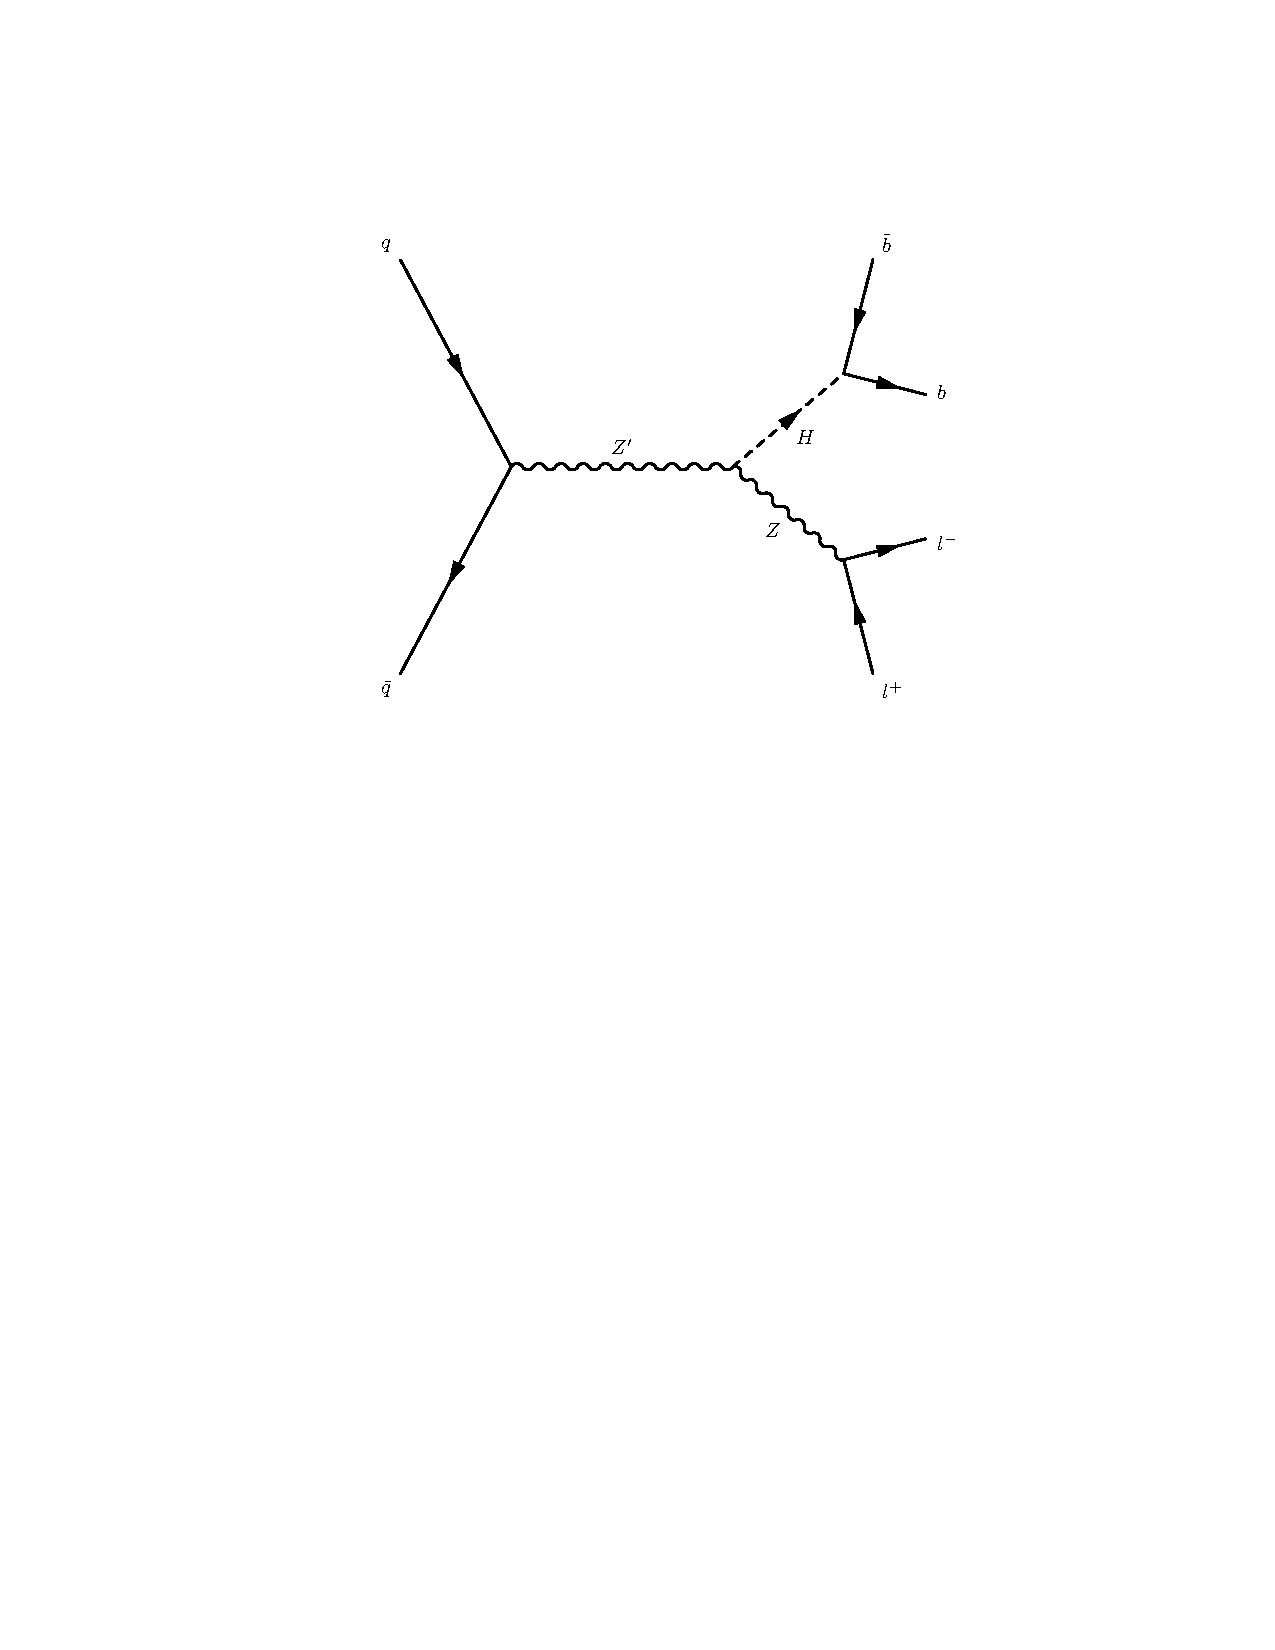
\includegraphics[width=1\textwidth,trim=0 400 0 100,clip=true]{Figures/feymann/qqZpZHllbb.pdf}
  \caption{Feymann diagram of the production of the heavy vector $Z'$, decaying into a $Z$ boson and a Higgs boson. The $Z$ boson further decays into two charged leptons, while the Higgs further decays into two $b$ quarks.}
  \label{fig:fey_signal}
\end{figure}

\section{Theoretical Motivations}

In the Standard Model (SM), the generation of masses for the weak gauge bosons ($W^\pm$ and $Z$) through electroweak symmetry breaking (EWSB) can be explained by the Higgs mechanism~\cite{PhysRevLett.13.508}. The mechanism was confirmed by the ATLAS and CMS experiments~\cite{Aad:2012tfa,Chatrchyan:2012xdj,Chatrchyan:2013lba} at the CERN 50 years after the theory has been proposed.

However, the discovered Higgs boson with mass of 125 GeV is much lighter than the Planck energy, which suggests that the SM may be incomplete. Various theories postulate the existence of new heavy resonances that couple to the SM bosons in an attempt to solve the hierarchy problem or naturalness problem. Some common models include the Little Higgs models~\cite{Han:2003wu,Perelstein:2005ka} and strongly coupled Composite Higgs~\cite{Contino:2011np,Marzocca:2012zn}. 

Various models can be generalized in the Heavy Vector Triplet (HVT) framework~\cite{Pappadopulo:2014qza}, which is a simplified approach based on a phenomenological Lagrangian. In the Simplified Model, only the relevant couplings and mass parameters are retained. The reason for this is that resonant searches are typically not sensitive to all the free parameters of the specific model, but only to those parameters that are related to the resonance mass and the interactions involved in its decay and production.

\subsection{Heavy Vector Triplet} \label{sec:hvtmodel}

Consider a heavy vector boson $V_\mu^a$, $a$ = 1,2,3, the simplified Lagrangian is described as
\begin{equation} \label{eq:simpleLag}
  \begin{aligned}
    \mathcal{L}_V = &-\frac{1}{4}D_{[\mu}V_{\nu]}^aD^{[\mu}V^{\nu]a}+\frac{m_V^2}{2}V_\mu^aV^{\mu a}\\
    &+ig_Vc_HV_\mu^aH^\dagger\tau^a\bar{D}^\mu H+\frac{g^2}{g_V}c_FV_\mu^a\sum\limits_{f}\bar{f}_L\gamma^\mu\tau^af_L\\
    &+\textup{quadrilinear terms}
  \end{aligned}
\end{equation}

The first term\footnote{The term \(D_{[\mu}V_{\nu]}^a = D_\mu V_\nu^a - D_\nu V_\mu^a\), where \(D_\mu V_\nu^a = \partial_\mu V_\nu^a + g\varepsilon^{abc}W_\mu^bV_\nu^c\).} in Eq.~\ref{eq:simpleLag} describes the interactions of $V$ with the SM weak bosons. The second term in the equation is the interactions of $V$ with itself, where the mass parameter $m_V$ does not coincide with the physical mass of the resonances. The third and fourth terms of the equation contains the interactions of $V$ with the Higgs current\footnote{The Higgs current term \(iH^\dagger\tau^a\bar{D}^\mu H = iH^\dagger\tau^aD^\mu H - iD^\mu H^\dagger\tau^aH\).} and with the SM left-handed fermionic currents\footnote{The fermionic currents \(\sum\bar{f}_L\gamma^\mu\tau^af_L\) involve the interactions of $V$ to leptons, light quarks and the third quarks family.}, respectively. The quadrilinear terms\footnote{The quadrilinear terms can be written as \[\frac{g_V}{2}c_{VVV}\varepsilon_{abc}V_\mu^aV_\nu^bD^{[\mu}V^{\nu]c} + g_V^2c_{VVHH}V_\mu^aV^{\nu a}H^\dagger H - \frac{g}{2}c_{VVW}\varepsilon_{abc}W^{\mu\nu a}V_\mu^bV_\nu^c.\]} do not contribute directly to $V$ decays and single production processes, therefore these terms can be disregarded.

In Eq.~\ref{eq:simpleLag}, besides the $SU$(2)$_L$ coupling constant $g$, another coupling constant $g_V$ is introduced to represent the strength of $V$ interactions. In addition, the term $c_H$ describes the $V$ interactions with the SM vector bosons and with the Higgs. Similarly, the term $c_F$ describes the $V$ interactions with fermions. They are expected to be of the order of unity in most models. 

\subsubsection*{Masses}

After the EWSB, only the photon stays massless due to the unbroken $U$(1)$_{EM}$, while the weak bosons acquire a mass and a mixing with heavy vector $V$. The mass matrix of the ($Z$, $V^0$) and the ($W^\pm$, $V^\pm$) are 
\begin{equation} \label{eq:matrixN}
  \mathcal{M}_N^2 =
  \begin{pmatrix}
    \hat{m}_Z^2 &
    c_H\xi\hat{m}_Z\hat{m}_V \\
    c_H\xi\hat{m}_Z\hat{m}_V &
    \hat{m}_V^2 \\
  \end{pmatrix}
\end{equation}
and
\begin{equation} \label{eq:matrixC}
  \mathcal{M}_C^2 =
  \begin{pmatrix}
    \hat{m}_W^2 &
    c_H\xi\hat{m}_W\hat{m}_V \\
    c_H\xi\hat{m}_W\hat{m}_V &
    \hat{m}_V^2 \\
  \end{pmatrix}
\end{equation}
respectively, where
\[\hat{m}_Z = \frac{e}{2\sin\theta_W\cos\theta_W}\hat{v}\]
\[\hat{m}_W = \cos\theta_W\hat{m}_Z\]
\[\hat{m}_V^2 = m_V^2 + g_V^2c_{VVHH}\hat{v}^2\]
\[\xi = \frac{g_V\hat{v}}{2\hat{m}_V}\]
Note that $e \approx \sqrt{4\pi/137}$, $\hat{v}$ is the Higgs field Vacuum Expectation Value, which has a value of 246 GeV, and $\theta_W$ is the weak mixing angle.

By taking the determinant of the mass matrices in Eq.~\ref{eq:matrixN} and Eq.~\ref{eq:matrixC}, the relation of the physical masses $M$ between charged and neutral heavy vectors are connected by $\theta_W$.
\begin{equation}
  m_W^2M_\pm^2 = \cos^2\theta_Wm_Z^2M_0^2
\end{equation}

In the experimental searches, the masses of new vectors should be at or above TeV scale, but the masses of SM bosons $m_{W,Z}$ should be preserved at about 100 GeV. A hierarchy in the mass spectrum is required to have
\begin{equation} \label{eq:massLimit}
  \frac{\hat{m}_{W,Z}}{\hat{m}_V} \sim \frac{m_{W,Z}}{M_{\pm,0}} \ll 1
\end{equation}

Under the limit in Eq.~\ref{eq:massLimit}, by expanding the determinant of the mass matrices in Eq.~\ref{eq:matrixN} and Eq.~\ref{eq:matrixC}, a simple approximate expressions for $m_W$ and $m_Z$ are given by
\[m_Z^2 \approx \hat{m}_Z^2(1-c_H^2\xi^2)\]
\[m_W^2 \approx \hat{m}_W^2(1-c_H^2\xi^2)\]
Since $\hat{m}_W = \cos\theta_W\hat{m}_Z$, the $W$-$Z$ mass ratio is given by 
\begin{equation} \label{eq:weakMass}
  \frac{m_W^2}{m_Z^2} \simeq \cos^2\theta_W
\end{equation}

Experimentally, the value of $\cos^2\theta_W$ is about 0.77. The charged and neutral $V$s are degenerated by
\begin{equation} \label{eq:hvtMass}
  M_\pm^2 = M_0^2 (1+\mathcal{O}(\%))
\end{equation}

It is clear that the mass splitting of charged and neutral states of $V$ is small enough to be ignored. This implies that the two states have comparable production rates.

\subsubsection*{Decay Widths}

Given that the mixing angles between weak bosons and $V$ are small due to the hierarchy in the mass spectrum, the couplings of the neutral and charged $V$ to left- and right-handed fermion chiralities can be written as
\begin{equation} \label{eq:LRcoupling}
  \begin{cases}
    g_L^N \simeq\frac{g^2}{g_V}\frac{c_F}{2}, \quad g_R^N \simeq 0 \\
    g_L^C \simeq\frac{g^2}{g_V}\frac{c_F}{\sqrt{2}}, \quad g_R^C = 0
  \end{cases}
\end{equation}
The ($g_{L,R}^{W,Z}$)$_{SM}$ in the Eq.~\ref{eq:LRcoupling} is the ordinary SM $W$ and $Z$ couplings with a normalization of $g_L^W = g/\sqrt{2}$. The $g$ is electroweak coupling which has a value of 0.65.

The decay width $\Gamma$ for fermionic channels can be written as
\begin{equation} \label{eq:fermionWidth}
  \Gamma_{V_\pm\rightarrow f\bar{f}'} \simeq 2\Gamma_{V_0\rightarrow f\bar{f}} \simeq N_c[f](\frac{g^2c_F}{g_V})^2\frac{M_V}{48\pi}
\end{equation}
where $N_c[f]$ is the number of colors (3 for di-quarks and 1 for di-leptons). The parameters $c_F={c_l,c_q,c_3}$ control the relative branching ratios (BR) to leptons, light quarks and the third family quarks.

The decay width for bosonic channels are
\begin{equation} \label{eq:bosonWidth}
  \Gamma_{V_0\rightarrow W_L^+W_L^-}\simeq\Gamma_{V_\pm\rightarrow W_L^\pm Z_L}\simeq\Gamma_{V_0\rightarrow Z_Lh}\simeq\Gamma_{V_\pm\rightarrow W_L^\pm h}\simeq\frac{g_V^2c_H^2M_V}{192\pi}[1+\mathcal{O}(\xi^2)]
\end{equation}
The channels that are not reported in the Eq.~\ref{eq:fermionWidth} and Eq.~\ref{eq:bosonWidth} are either forbidden or suppressed.

Since the $M_V$ is in the order of TeV scale, the $\xi$ should be very small. In this case, for a given resonance mass, the decay widths are fixed by the couplings $g^2c_F/g_V$ and $g_Vc_H$. The BRs and the production rate are controlled by the two parameters $g^2c_F/g_V$ and $g_Vc_H$.

\begin{figure}[t]
  \centering
  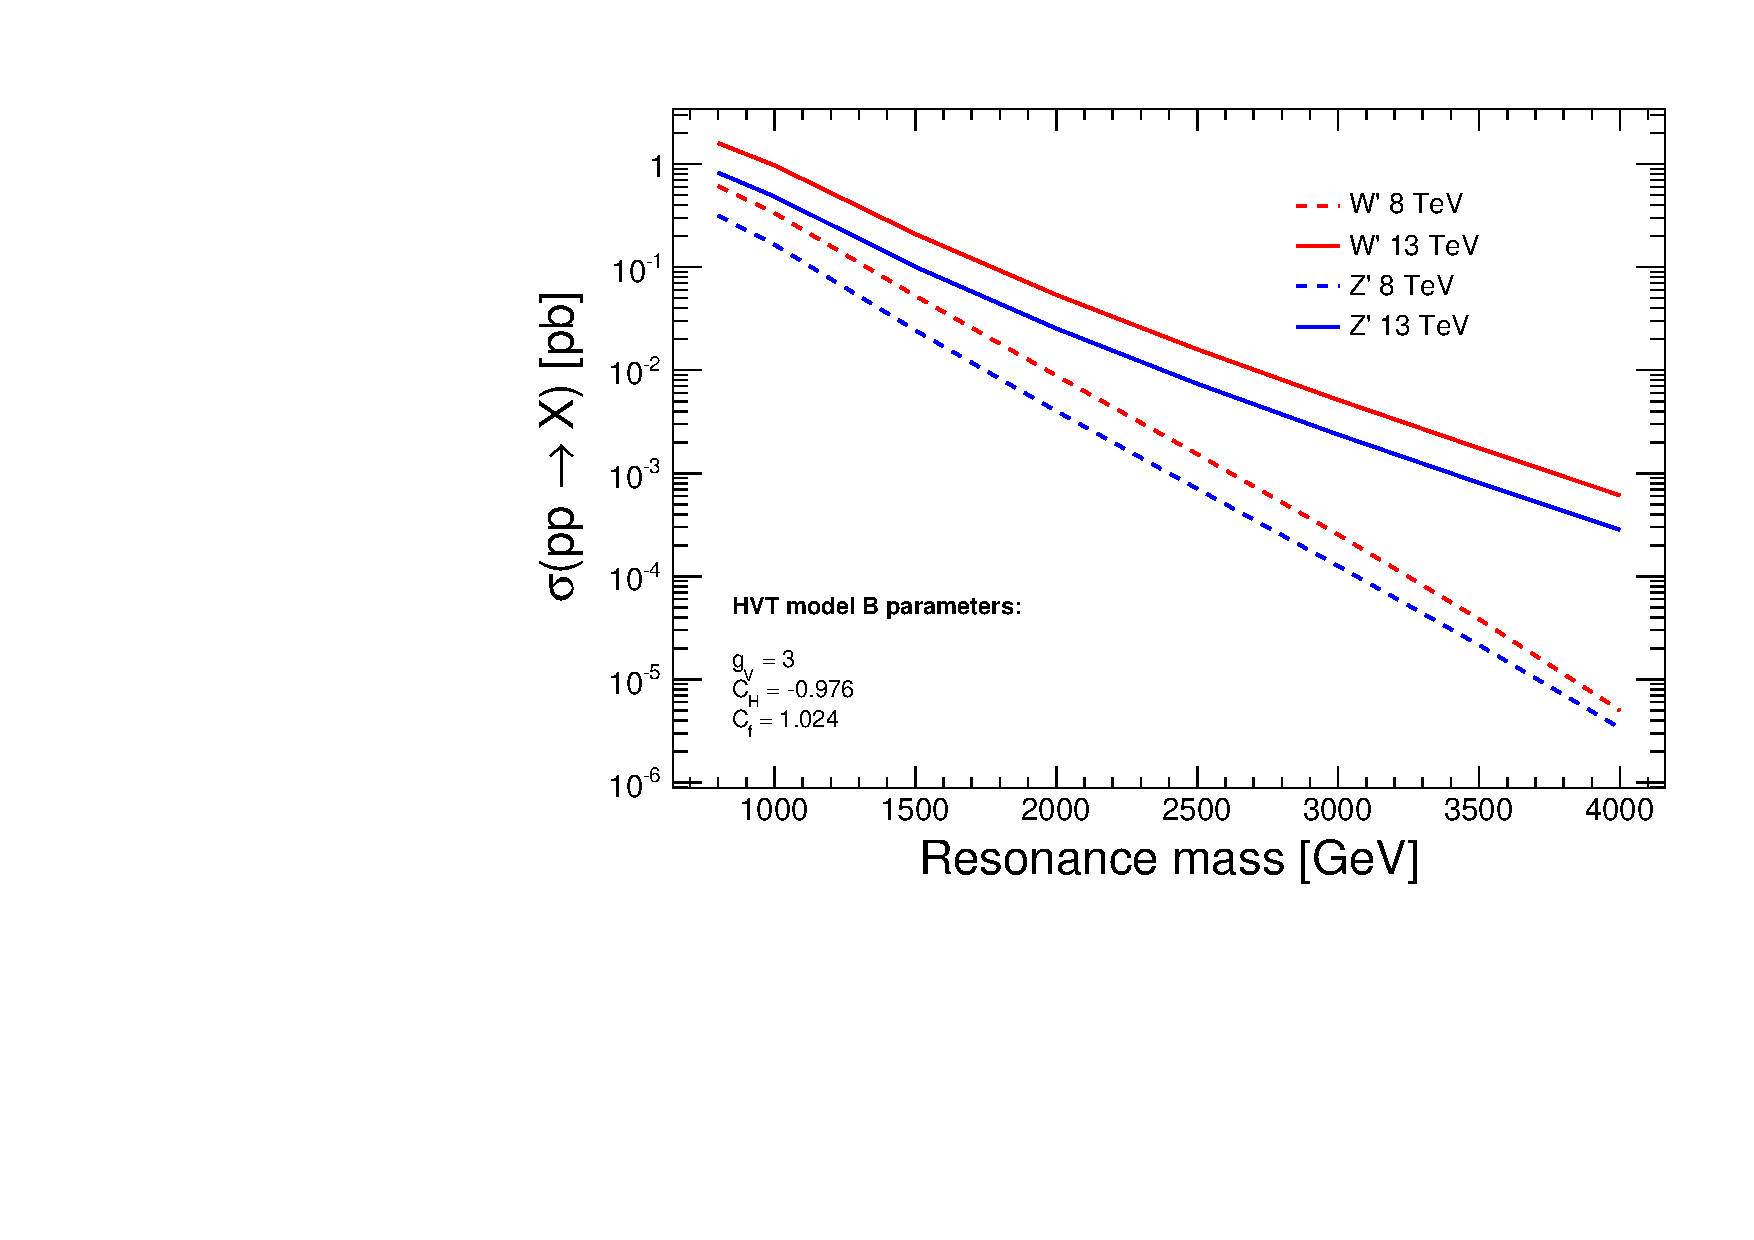
\includegraphics[width=0.55\textwidth]{Figures/hvt-xsec.pdf}
  \caption{Theoretical production cross section as a function of resonance mass for HVT Minimal Composite Higgs Model.}
  \label{fig:hvt_xsec}
\end{figure}

\subsection{Explicit Model} \label{sec:modelb}

It is now clear that the explicit model can be entirely described in terms of the two couplings $g^2c_F/g_V$ and $g_Vc_H$ and the mass $M_V$ with a good approximation~\cite{Pappadopulo:2014qza}.

Consider a strongly coupled scenario, so called Minimal Composite Higgs Model, where the Higgs doublet emerges from the spontaneous symmetry breaking of a global $SO$(5) symmetry to an $SO$(4) subgroup. In this scenario, the parameters $c_H$ and $c_F$ are fixed, \[c_H \sim -1, \quad c_F \sim 1\]

In addition, $g_V \gtrsim$ 3 is set to represent the strong coupling. In this case, the dominant BRs are bosonic decays due to $g_Vc_H \simeq -g_V$ in Eq.~\ref{eq:bosonWidth}, while the fermionic decays are extremely suppressed due to $g^2c_F/g_V \simeq g^2/g_V$ in Eq.~\ref{eq:fermionWidth}.

The results of this model is particularly interesting for the present search, since it predicts signal cross sections in the order of $fb$ for resonances up to 2$\sim$3 TeV (Figure~\ref{fig:hvt_xsec}), branching ratios to vector bosons close to the unity (Figure~\ref{fig:hvt_brs}), and thus being accessible at the LHC Run-II.

If the coupling is very large (for example $g_V$ = 8), the total width will be increased since the width of decays to dibosons grows with $g_V$ from Eq.~\ref{eq:bosonWidth}. But a very large coupling leads to an extremely broad resonance, which is not interesting to the experimental searches for a narrow resonance. Therefore, the $g_v$ has been constrained by $g_V \lesssim 4\pi$.

\begin{figure}[t]
  \centering
  \begin{tabular}{cc}
    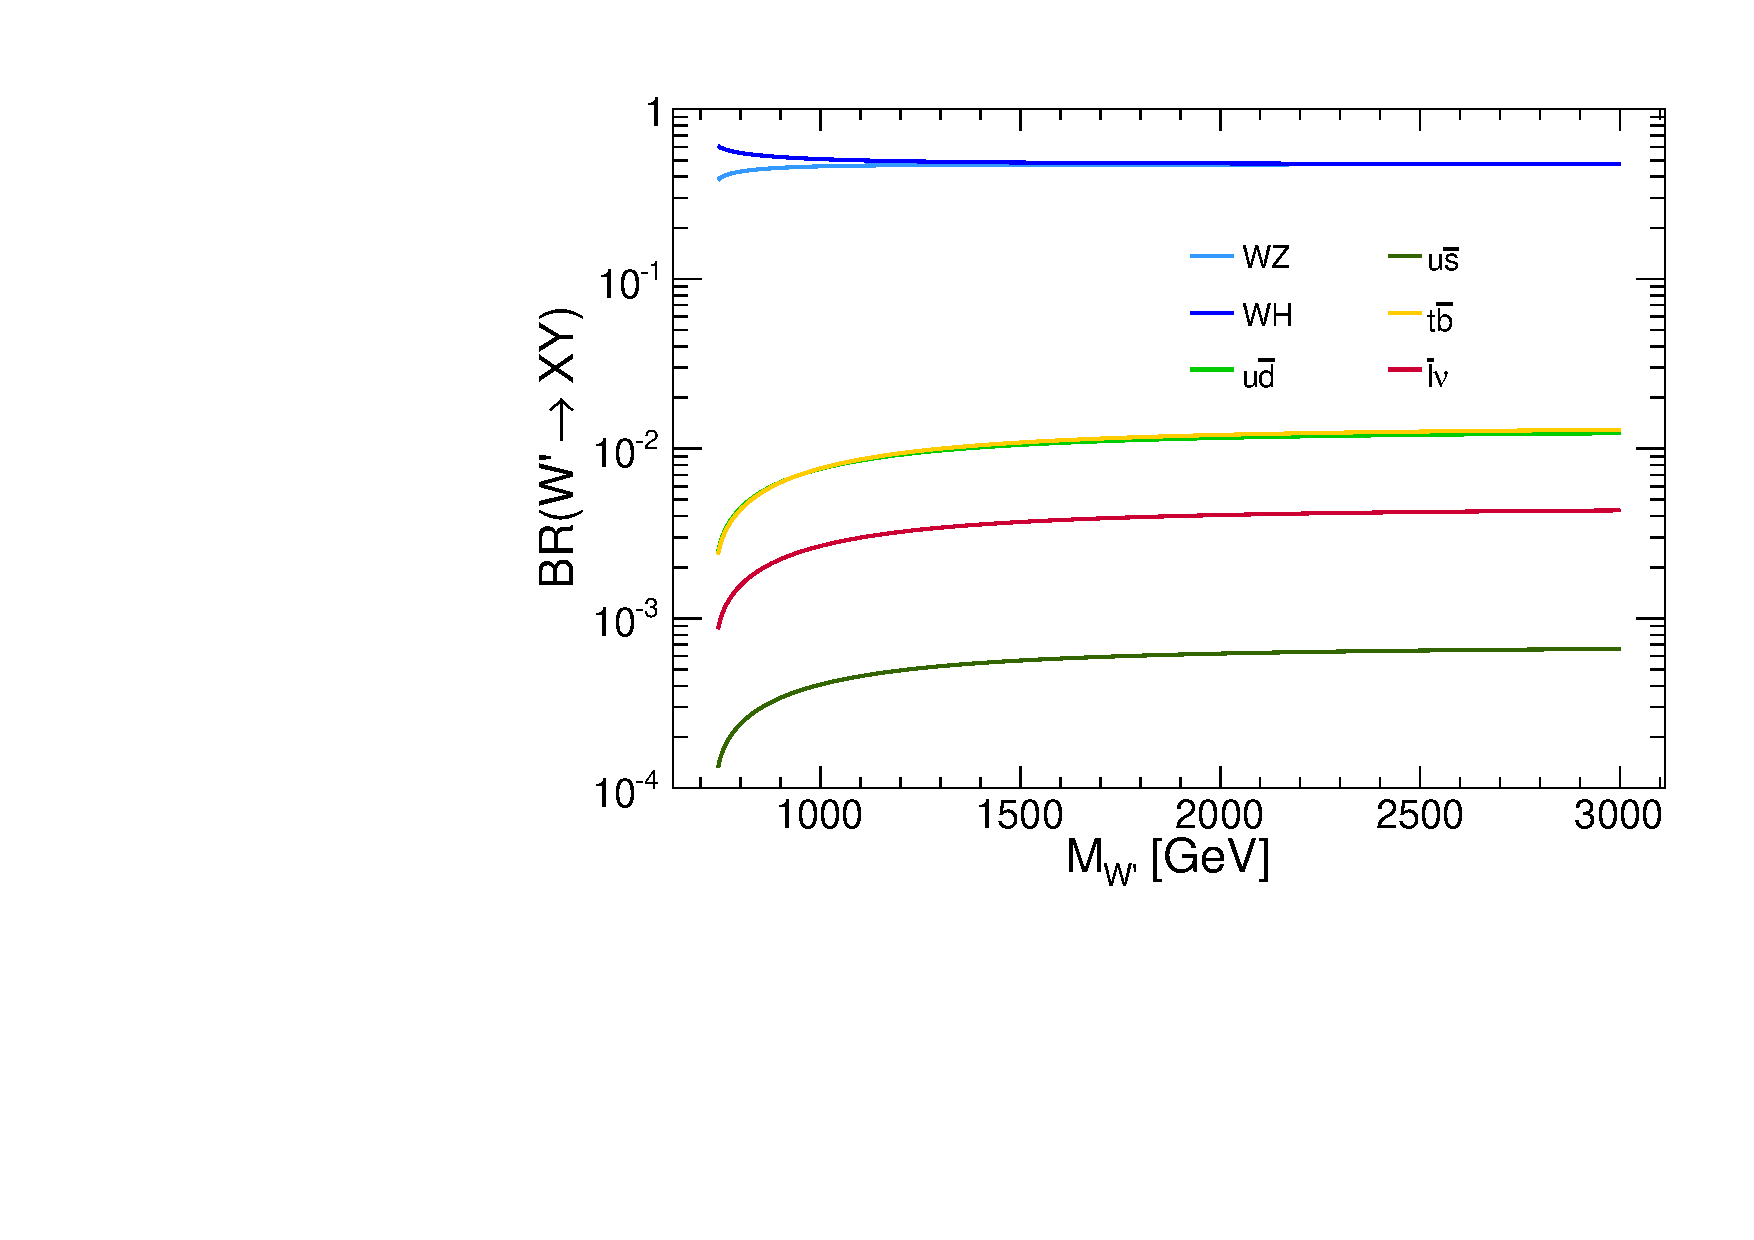
\includegraphics[width=0.5\textwidth]{Figures/hvt-wp-brs.pdf} &
    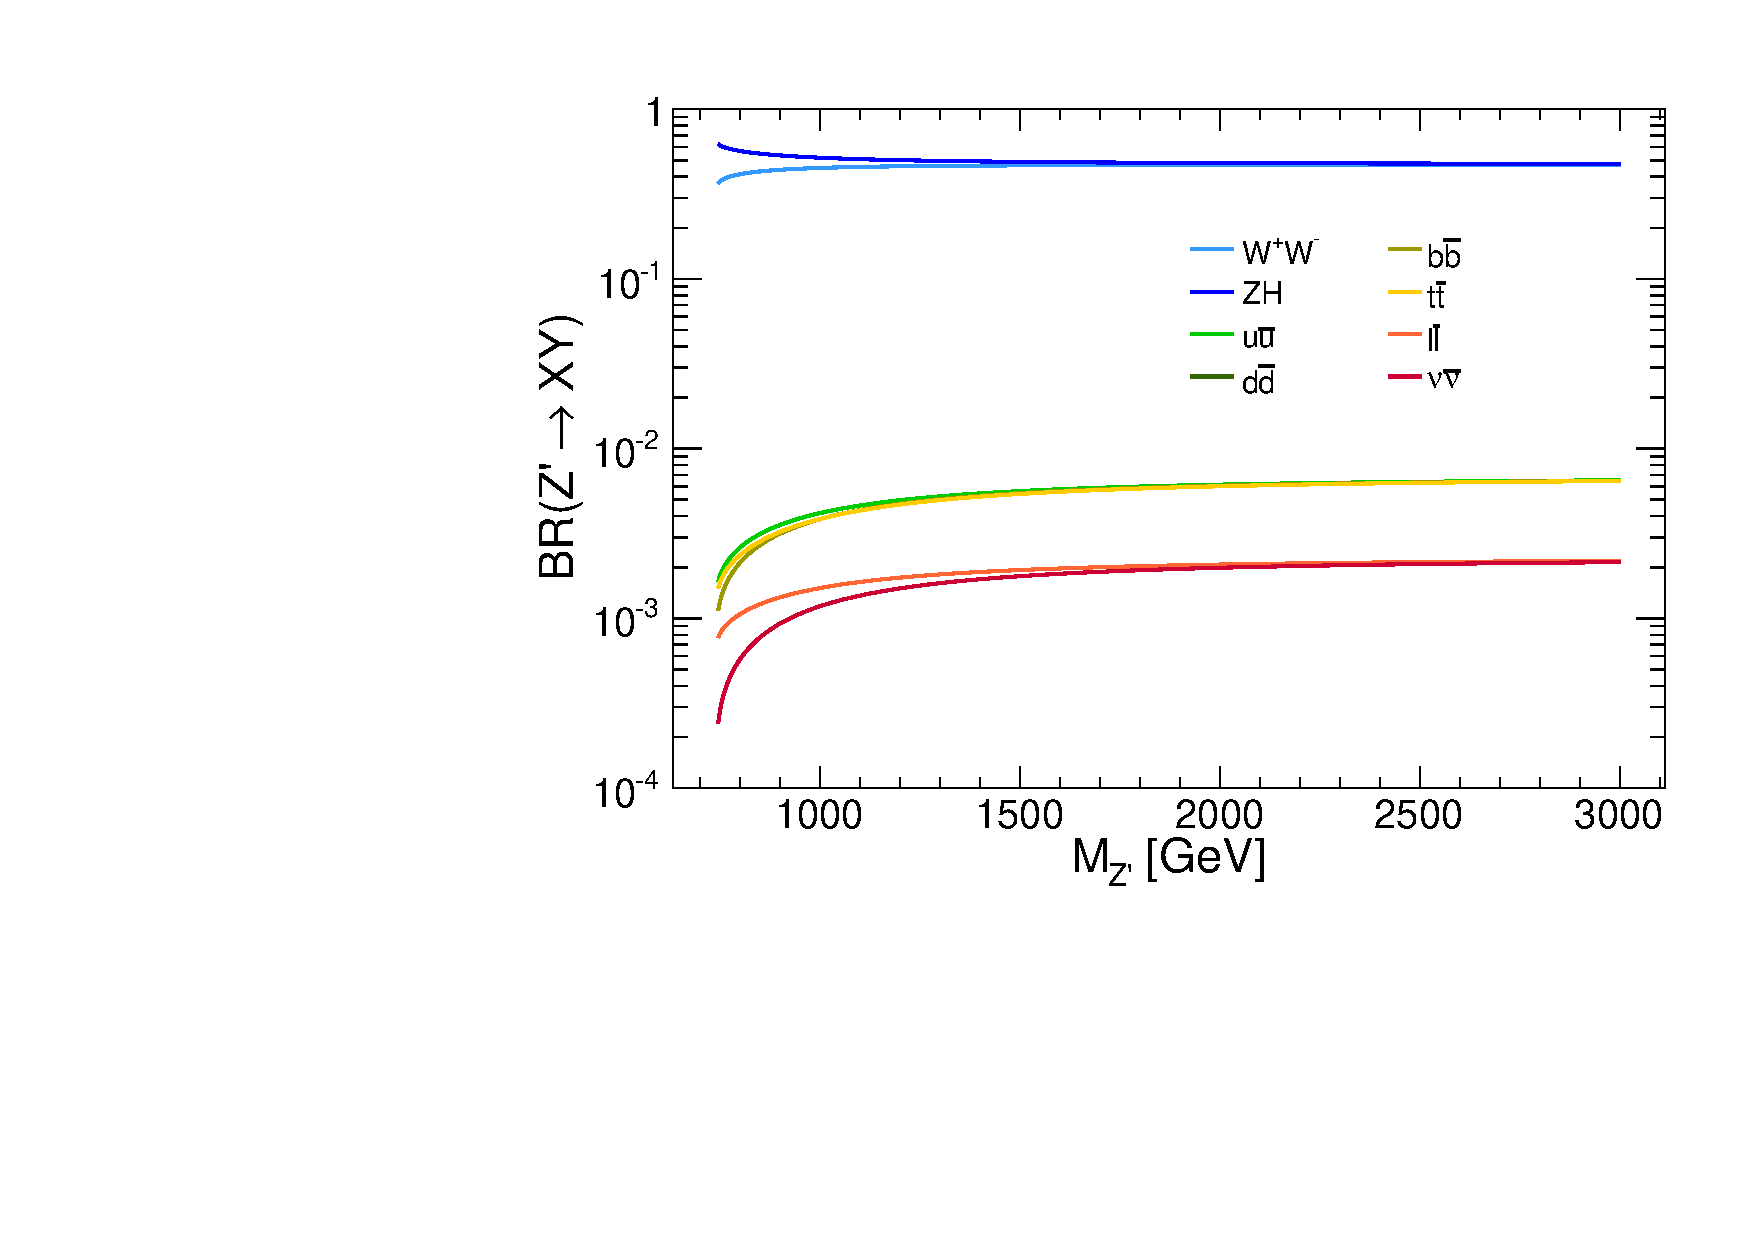
\includegraphics[width=0.5\textwidth]{Figures/hvt-zp-brs.pdf} \\
  \end{tabular}
  \caption{Branching ratios as a function of the resonance mass for a W' (left) and Z' (right) in the HVT Minimal Composite Higgs Model.}
  \label{fig:hvt_brs}
\end{figure}
 
%\include{Chapters/Chapter3}
%\include{Chapters/Chapter4} 
%\include{Chapters/Chapter5} 

%----------------------------------------------------------------------------------------
%	THESIS CONTENT - APPENDICES
%----------------------------------------------------------------------------------------

\appendix % Cue to tell LaTeX that the following "chapters" are Appendices

% Include the appendices of the thesis as separate files from the Appendices folder
% Uncomment the lines as you write the Appendices

%\include{Appendices/AppendixA}
%\include{Appendices/AppendixB}
%\include{Appendices/AppendixC}

%----------------------------------------------------------------------------------------
%	BIBLIOGRAPHY
%----------------------------------------------------------------------------------------

\printbibliography[heading=bibintoc]

%----------------------------------------------------------------------------------------

\end{document}  
